% LaTeX source for ``Python for Informatics: Exploring Information''
% Copyright (c)  2010-  Charles R. Severance, All Rights Reserved

\chapter{Execução Condicional}
%\chapter{Conditional execution}

\section{Expressões booleanas}
%\section{Boolean expressions}

\index{Expressão booleana}
%\index{boolean expression}

\index{expressão!booleana}
%\index{expression!boolean}

\index{operador lógico}
%\index{logical operator}

\index{operador!lógico}
%\index{operator!logical}

Uma {\bf expressão booleana} é uma expressão que é true 
ou false.  Os seguintes exemplos usam o 
operador {\tt ==}, que compara dois operadores e produz
{\tt True} se eles forem iguais e {\tt False} caso contrário:

% A {\bf boolean expression} is an expression that is either true
% or false.  The following examples use the 
% operator {\tt ==}, which compares two operands and produces
% {\tt True} if they are equal and {\tt False} otherwise:

\beforeverb
\begin{verbatim}
>>> 5 == 5
True
>>> 5 == 6
False
\end{verbatim}
\afterverb
%

{\tt True} e {\tt False} são valores
especiais que pertencem ao tipo {\tt bool}; eles não são strings:
% {\tt True} and {\tt False} are special
% values that belong to the type {\tt bool}; they are not strings:

\index{True valor especial}
\index{False valor especial}
\index{especial valor!True}
\index{especial valor!False}
\index{bool tipo}
\index{tipo!bool}

% \index{True special value}
% \index{False special value}
% \index{special value!True}
% \index{special value!False}
% \index{bool type}
% \index{type!bool}

\beforeverb
\begin{verbatim}
>>> type(True)
<type 'bool'>
>>> type(False)
<type 'bool'>
\end{verbatim}
\afterverb
%

O operador {\tt ==} é um dos {\bf operadores de comparação}; os
outros são:
% The {\tt ==} operator is one of the {\bf comparison operators}; the
% others are:

\beforeverb
\begin{verbatim}
      x != y               # x não é igual a y
      x > y                # x é maior que y
      x < y                # x é menor que y
      x >= y               # x é maior ou igual a y
      x <= y               # x é menor ou igual a y
      x is y               # x é o mesmo que y
      x is not y           # x não é o mesmo que y
\end{verbatim}
\afterverb

% \beforeverb
% \begin{verbatim}
%       x != y               # x is not equal to y
%       x > y                # x is greater than y
%       x < y                # x is less than y
%       x >= y               # x is greater than or equal to y
%       x <= y               # x is less than or equal to y
%       x is y               # x is the same as y
%       x is not y           # x is not the same as y
% \end{verbatim}
% \afterverb
%

Embora estas operações sejam provavelmente familiar para você, os simbolos
Python são diferentes dos símbolos matemáticos para a mesma 
operação.  Um erro comum
é usar um único sinal de igual ({\tt =}) em vez de um sinal de igual duplo
({\tt ==}).  Lembre-se que o {\tt =} é um operador de atribuição e 
{\tt ==} é um operador de comparação. Não existe tal coisa como
{\tt =<} ou {\tt =>}.

% Although these operations are probably familiar to you, the Python
% symbols are different from the mathematical symbols for the same
% operations.  A common error
% is to use a single equal sign ({\tt =}) instead of a double equal sign
% ({\tt ==}).  Remember that {\tt =} is an assignment operator and
% {\tt ==} is a comparison operator.   There is no such thing as
% {\tt =<} or {\tt =>}.

\index{operador de comparação}
%\index{comparison operator}

\index{operador!comparação}
%\index{operator!comparison}

\section {Operador Lógico}
\index{operador lógico}
\index{operador!lógico}
% \section {Logical operators}
% \index{logical operator}
% \index{operator!logical}

Existem três {\bf operadores lógicos}: {\tt and}, {\tt
or}, and {\tt not}. A semântica (significado) destes operadores é
semelhante ao seu significado em inglês. Por exemplo,

% There are three {\bf logical operators}: {\tt and}, {\tt
% or}, and {\tt not}.  The semantics (meaning) of these operators is
% similar to their meaning in English.  For example,

{\tt x > 0 and x < 10} 

só é verdade se {\tt x} for maior que 0
\emph{e} menor que 10.

% is true only if {\tt x} is greater than 0
% \emph{and} less than 10.

\index{and operador}
\index{or operador}
\index{not operador}
\index{operador!and}
\index{operador!or}
\index{operador!not}

% \index{and operator}
% \index{or operator}
% \index{not operator}
% \index{operator!and}
% \index{operator!or}
% \index{operator!not}

{\tt n\%2 == 0 or n\%3 == 0} é verdadeiro se \emph{qualquer} uma das condições
é verdadeira, isto é, se o número é divisível por 2 \emph{ou} 3.

% {\tt n\%2 == 0 or n\%3 == 0} is true if \emph{either} of the conditions
% is true, that is, if the number is divisible by 2 \emph{or} 3.

Finalmente, o operador {\tt not} nega uma expressão
booleana, então {\tt not (x > y)} é verdadeiro se {\tt x > y} é falso;
isto é, se {\tt x} é menor do que ou igual a {\tt y}.

% Finally, the {\tt not} operator negates a boolean
% expression, so {\tt not (x > y)} is true if {\tt x > y} is false;
% that is, if {\tt x} is less than or equal to {\tt y}.

Rigorosamente falando, os operandos dos operadores logicos devem ser
expressões booleanas, mas Python não é muito rigoroso.
Qualquer numero diferente de zero é interpretado como ``verdadeiro.''

% Strictly speaking, the operands of the logical operators should be
% boolean expressions, but Python is not very strict.
% Any nonzero number is interpreted as ``true.''

\beforeverb
\begin{verbatim}
>>> 17 and True
True
\end{verbatim}
\afterverb
%
Esta flexibilidade pode ser útil, mas existem algumas sutilezas que
podem confundir o Python. Você pode querer evitá-los até
você ter certeza que sabe o que está fazendo.

% This flexibility can be useful, but there are some subtleties to
% it that might be confusing.  You might want to avoid it until
% you are sure you know what you are doing.

\section{Execução condicional}
\label{execucao condicional}
% \section{Conditional execution}
% \label{conditional execution}

\index{declaração condicional}
\index{declaração!condicional}
\index{se declaração}
\index{declaração!se}
\index{execução condicional}
% \index{conditional statement}
% \index{statement!conditional}
% \index{if statement}
% \index{statement!if}
% \index{conditional execution}

Para escrever programas úteis, quase sempre precisamos da capacidade
para verificar as condições e mudar o comportamento do programa
em conformidade.  {\bf Instruções condicionais} nos dão essa capacidade. A
forma mais simples é a instrução {\tt if}:

% In order to write useful programs, we almost always need the ability
% to check conditions and change the behavior of the program
% accordingly.  {\bf Conditional statements} give us this ability.  The
% simplest form is the {\tt if} statement:

\beforeverb
\begin{verbatim}
if x > 0 :
    imprima 'x é positivo'
\end{verbatim}
%\begin{verbatim}
%if x > 0 :
%    print 'x is positive'
%\end{verbatim}
\afterverb
%

A expressão booleana depois da declaração {\tt if} é
chamado de {\bf condição}. Terminamos a instrução {\tt if}
com um caractere dois pontos (:) e a(s) linha(s)
após a instrução if são identadas.

% The boolean expression after the {\tt if} statement is
% called the {\bf condition}.  We end the {\tt if} 
% statement with a colon character (:) and the line(s) 
% after the if statement are indented.  

\beforefig
\centerline{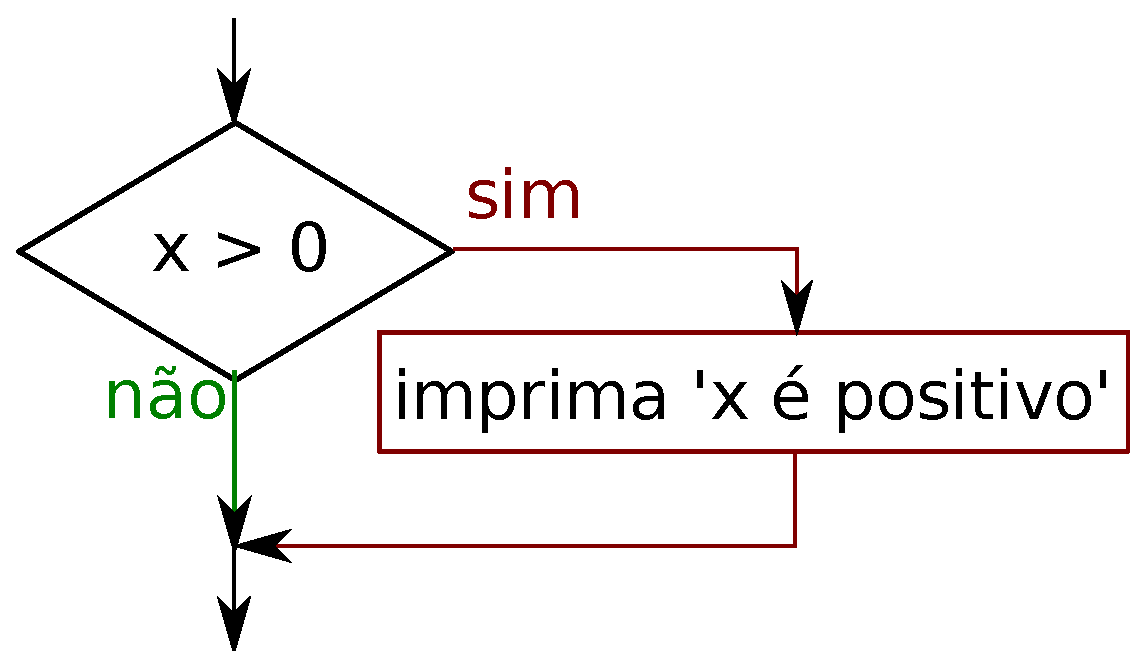
\includegraphics[height=1.75in]{figs2/if.eps}}
\afterfig

Se a condição lógica é verdadeira, então a instrução
identada é executada. Se a condição lógica é
falsa, a instrução identada é ignorada.

% If the logical condition is true, then the indented
% statement gets executed.  If the logical condition is 
% false, the indented statement is skipped.

\index{condição}
\index{declaração composta}
\index{declaração!composta}
% \index{condition}
% \index{compound statement}
% \index{statement!compound}

Instruções {\tt if} têm a mesma estrutura que as definições de funções
ou loops {\tt for} \footnote{Vamos aprender sobre as funções no Capítulo 4
e loops no Capítulo 5.}. A instrução é composta por uma linha de cabeçalho
que termina com o caractere dois pontos (:)
seguido por um bloco identado. Instruções como esta são
chamadas {\bf declarações compostas} porque elas são compostas
por mais de uma linha.

% {\tt if} statements have the same structure as function definitions
% or {\tt for} loops\footnote{We will learn about functions in Chapter 4
% and loops in Chapter 5.}.The statement consists of a header line
% that ends with the colon character (:) 
% followed by an indented block.  Statements like this are
% called {\bf compound statements} because they stretch 
% across more than one line.

Não há limite para o número de intruções que podem aparecer 
no corpo, mas deve haver pelo menos uma.
Às vezes, é util ter um corpo sem instruções (usualmente
como um corpo pacificador para o código que você não tenha escrito até o momento). Nesse
caso, você pode usar a instrução {\tt pass}, que não faz nada.

% There is no limit on the number of statements that can appear in
% the body, but there must be at least one.
% Occasionally, it is useful to have a body with no statements (usually
% as a placekeeper for code you haven't written yet).  In that
% case, you can use the {\tt pass} statement, which does nothing.

\index{instrução pass}
\index{instrução!pass}
%\index{pass statement}
%\index{statement!pass}

\beforeverb
\begin{verbatim}
if x < 0 :
    pass          # precisa lidar com valores negativos!
\end{verbatim}
%\begin{verbatim}
%if x < 0 :
%    pass          # need to handle negative values!
%\end{verbatim}
\afterverb
%
Se você digitar um {\tt if} no interpretador Python, o prompt vai se modificar
de três sinais >>> para três pontos ... para indicar que você está no meio de um bloco de
declarações, como mostrado abaixo:
% If you enter an {\tt if} statement in the Python interpreter, the prompt will change 
% from three chevrons to three dots to indicate you are in the middle of a block of
% statements, as shown below:

\beforeverb
\begin{verbatim}
>>> x = 3
>>> if x < 10:
...    print 'pequeno'
... 
Small
>>>
\end{verbatim}
%\begin{verbatim}
%>>> x = 3
%>>> if x < 10:
%...    print 'Small'
%... 
%Small
%>>>
%\end{verbatim}
\afterverb
%

\section{Execução alternativa}
\label{execucao alternativa}
%\section{Alternative execution}
%\label{alternative execution}

\index{execução alternativa}
\index{else keyword}
\index{keyword!else}
%\index{alternative execution}
%\index{else keyword}
%\index{keyword!else}

A segunda forma da instrução {\tt if} é a {\bf execução alternativa},
na qual há duas possibilidades e a condição determina
qual delas será executada. A sintaxe se parece com esta:

%A second form of the {\tt if} statement is {\bf alternative execution},
%in which there are two possibilities and the condition determines
%which one gets executed.  The syntax looks like this:

\beforeverb
\begin{verbatim}
if x%2 == 0 :
    print 'x ainda é'
else :
    print 'x é estranho'
\end{verbatim}
%\begin{verbatim}
%if x%2 == 0 :
%    print 'x is even'
%else :
%    print 'x is odd'
%\end{verbatim}
\afterverb
%

Se o resto da divisão de {\tt x} por 2 for 0, nós
sabemos que {\tt x} é divisível, e o programa exibe uma mensagem para esse
efeito. Se a condição for falsa, o segundo conjunto de instruções é
executado.

%If the remainder when {\tt x} is divided by 2 is 0, then we
%know that {\tt x} is even, and the program displays a message to that
%effect.  If the condition is false, the second set of statements is
%executed.  

\beforefig
\centerline{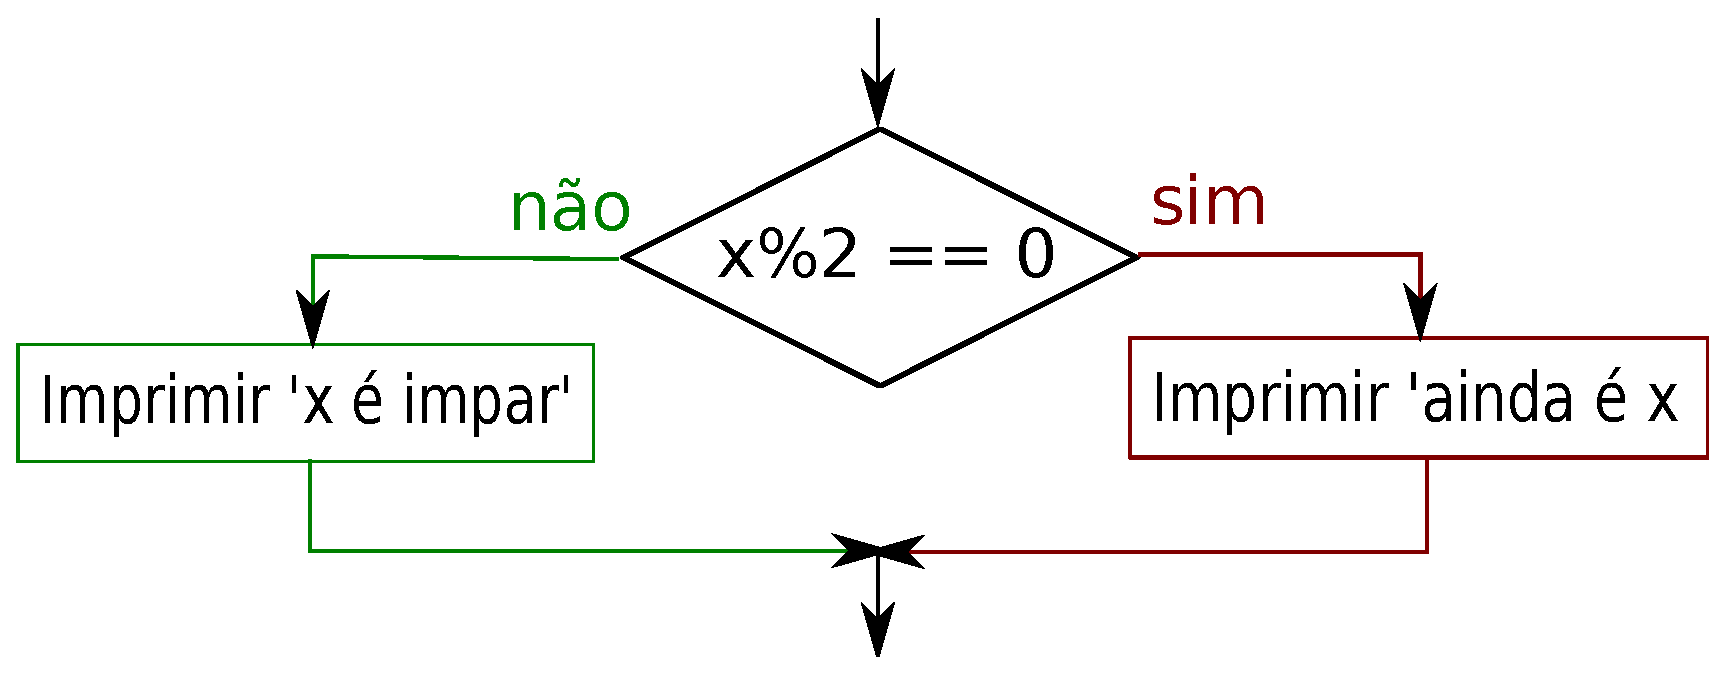
\includegraphics[height=1.75in]{figs2/if-else.eps}}
\afterfig

Uma vez que a condição deve ser verdadeira ou falsa, exatamente uma das
alternativas será executada. As alternativas são chamadas de
{\bf branches}, porque elas dividem o fluxo de execução.
%Since the condition must either be true or false, exactly one of
%the alternatives will be executed.  The alternatives are called
%{\bf branches}, because they are branches in the flow of execution.

\index{branch}

\section{Condicionais encadeadas}
%\section{Chained conditionals}
\index{chained conditional}
\index{conditional!chained}

Às vezes, há mais de duas possibilidades e precisamos de mais do que
duas condições. Uma maneira de expressar uma computação como essa é uma {\bf
condição encadeada}:
%Sometimes there are more than two possibilities and we need more than
%two branches.  One way to express a computation like that is a {\bf
%chained conditional}:

\beforeverb
\begin{verbatim}
if x < y:
    print 'x é menor que y'
elif x > y:
    print 'x é maior que y'
else:
    print 'x e y são iguais'
\end{verbatim}
\afterverb
%\begin{verbatim}
%if x < y:
%    print 'x is less than y'
%elif x > y:
%    print 'x is greater than y'
%else:
%    print 'x and y are equal'
%\end{verbatim}
\afterverb
%

{\tt elif} é uma abreviação de `` else if. '' Mais uma vez, exatamente uma
condição será executada.
%{\tt elif} is an abbreviation of ``else if.''  Again, exactly one
%branch will be executed.  

\beforefig
\centerline{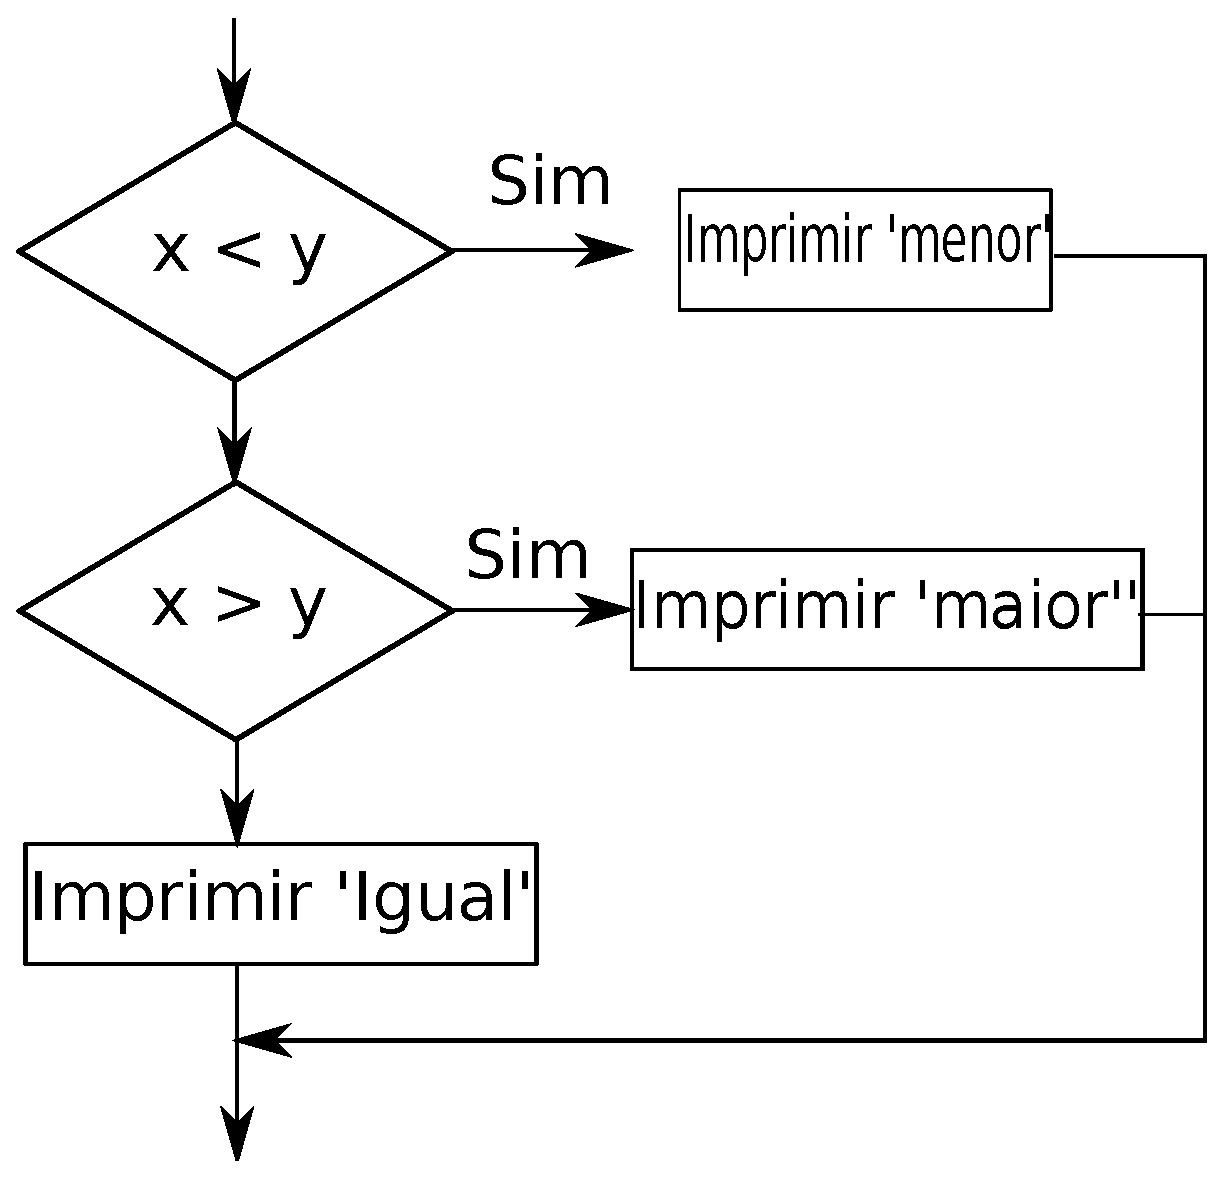
\includegraphics[height=3.00in]{figs2/elif.eps}}
\afterfig

Não há limite para o número de instruções {\tt
elif}. Se houver uma cláusula {\tt else}, ela deve estar no final,
mas só pode existir uma única instrução deste tipo.

%There is no limit on the number of {\tt
%elif} statements.  If there is an {\tt else} clause, it has to be
%at the end, but there doesn't have to be one.

\index{elif keyword}
\index{keyword!elif}
%\index{elif keyword}
%\index{keyword!elif}

\beforeverb
\begin{verbatim}
if choice == 'a':
    print 'Escolha ruim'
elif choice == 'b':
    print 'Boa escolha'
elif choice == 'c':
    print 'Perto, mas não correto'
\end{verbatim}
%\begin{verbatim}
%if choice == 'a':
%    print 'Bad guess'
%elif choice == 'b':
%    print 'Good guess'
%elif choice == 'c':
%    print 'Close, but not correct'
%\end{verbatim}
\afterverb
%

Cada condição é verificada em ordem. Se a primeira é falsa,
a próxima será avaliada, e assim por diante. Se um deles é
verdadeiro, o fluxo correspondente será executado, e a instrução
termina. Mesmo se mais do que uma condição for verdadeira, apenas o
primeiro fluxo verdadeiro é executado.

%Each condition is checked in order.  If the first is false,
%the next is checked, and so on.  If one of them is
%true, the corresponding branch executes, and the statement
%ends.  Even if more than one condition is true, only the
%first true branch executes.  


\section{Condicionais aninhados}
%\section{Nested conditionals}

\index{condicional aninhado}
\index{condicional!aninhado}
%\index{nested conditional}
%\index{conditional!nested}

Uma instrução condicional também pode ser aninhada dentro de outra. 
Nós poderíamos ter escrito o exemplo de três ramificações como a seguir:

%One conditional can also be nested within another.  We could have
%written the three-branch example like this:

\beforeverb
\begin{verbatim}
if x == y:
    print 'x e y são iguais'
else:
    if x < y:
        print 'x é menor que y'
    else:
        print 'x é maior que y'
\end{verbatim}
%\begin{verbatim}
%if x == y:
%    print 'x and y are equal'
%else:
%    if x < y:
%        print 'x is less than y'
%    else:
%        print 'x is greater than y'
%\end{verbatim}
\afterverb
%
A condicional externa contém duas ramificações. A
primeira ramificação contém uma instrução simples. A segunda ramificação
contém outra instrução {\tt if}, que contém duas ramificações
próprias. Aquelas duas ramificações são ambas instruções simples,
embora pudessem ter sido instruções condicionais também.

%The outer conditional contains two branches.  The
%first branch contains a simple statement.  The second branch
%contains another {\tt if} statement, which has two branches of its
%own.  Those two branches are both simple statements,
%although they could have been conditional statements as well.

\beforefig
\centerline{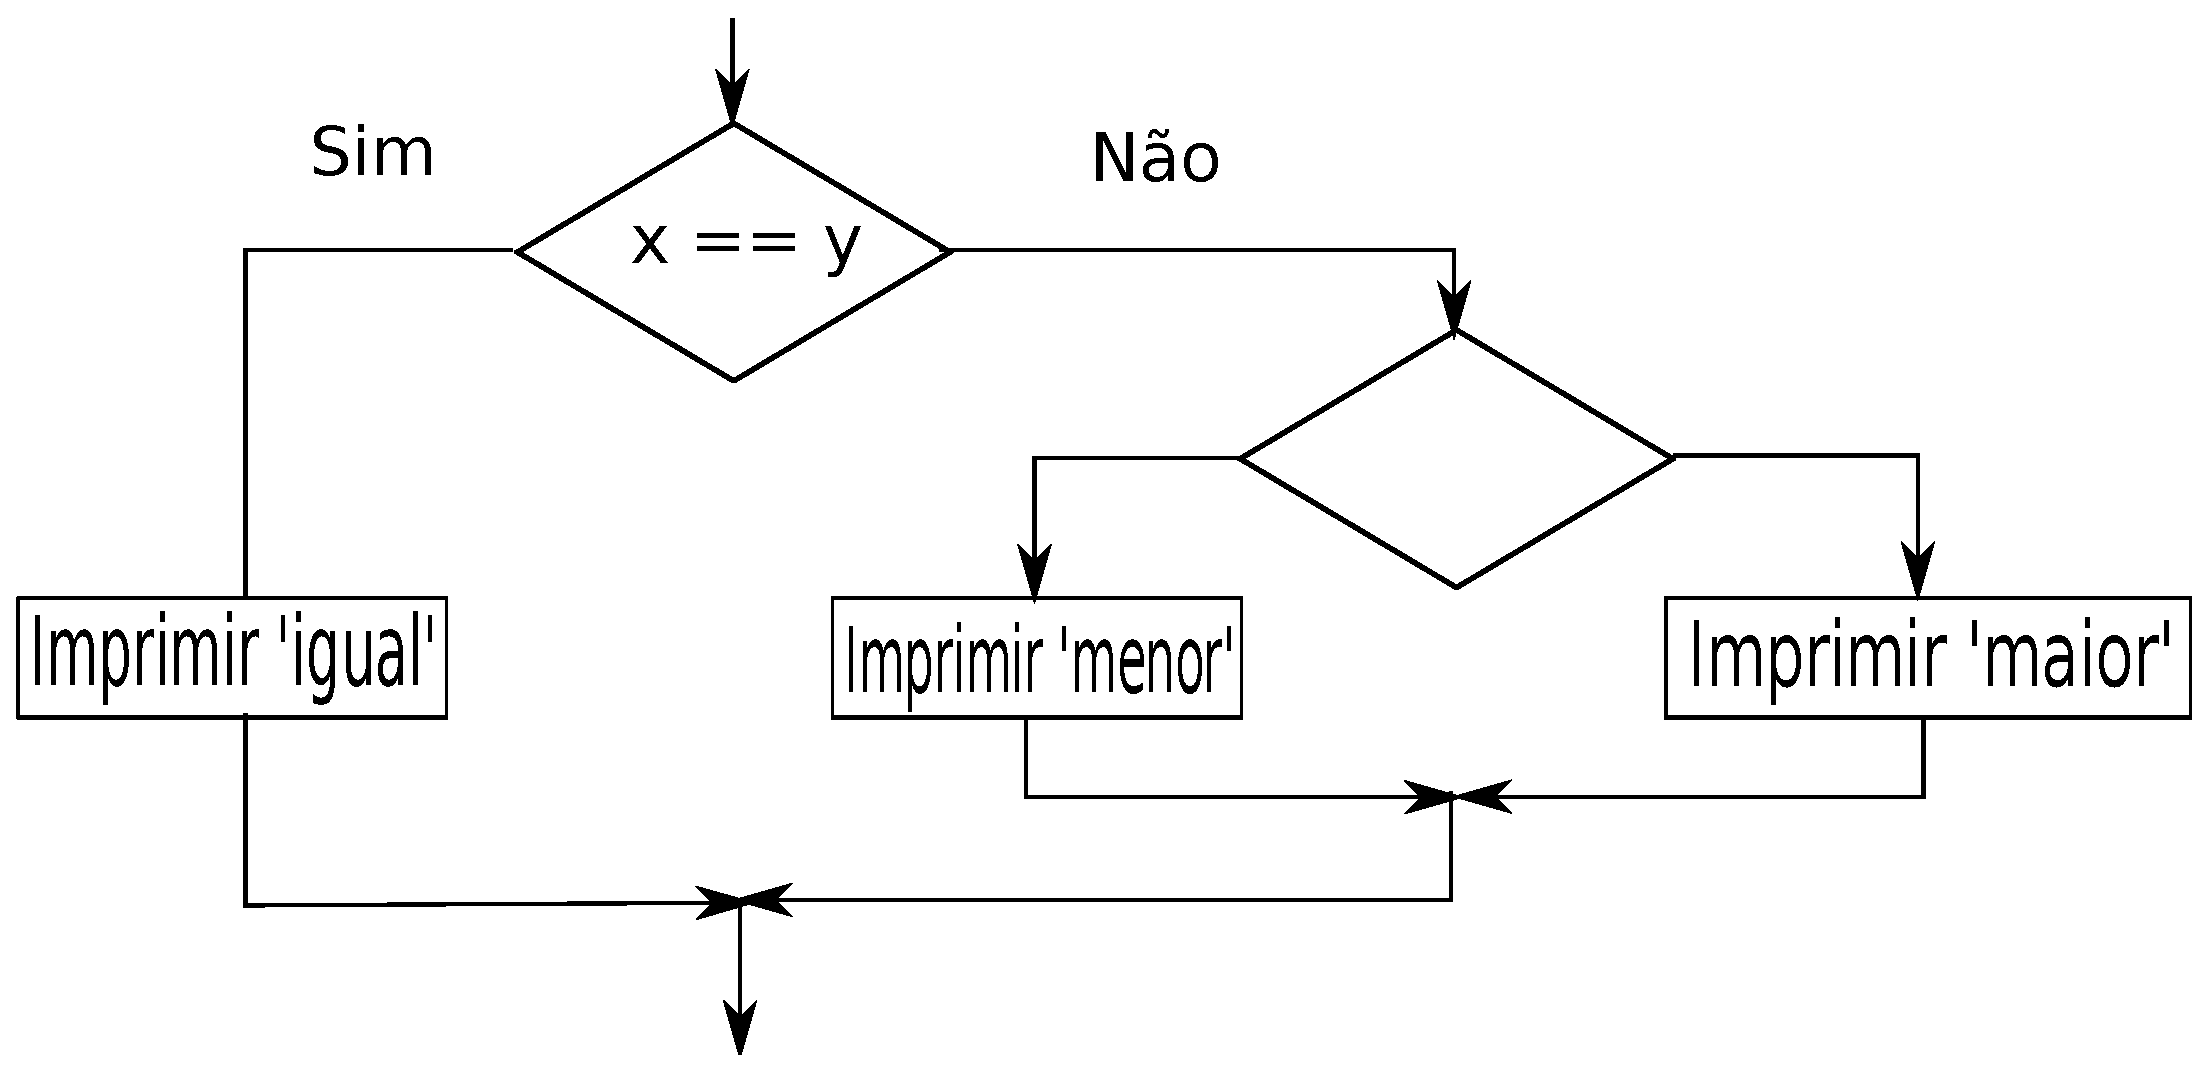
\includegraphics[height=2.50in]{figs2/nested.eps}}
\afterfig


Embora a identação das instruções torna a estrutura
visível, {\bf condicionais aninhadas} fica difícil de ler muito
rapidamente. Em geral, é uma boa idéia evitá-las sempre que possível.

%Although the indentation of the statements makes the structure
%apparent, {\bf nested conditionals} become difficult to read very
%quickly. In general, it is a good idea to avoid them when you can.


Os operadores lógicos muitas vezes fornecem uma maneira de simplificar as instruções
condicionais aninhadas. Por exemplo, podemos reescrever o código a seguir usando um
condicional simples:

%Logical operators often provide a way to simplify nested conditional
%statements.  For example, we can rewrite the following code using a
%single conditional:

\beforeverb
\begin{verbatim}
if 0 < x:
    if x < 10:
        print 'x é um número positivo de um dígito.'
\end{verbatim}
%\begin{verbatim}
%if 0 < x:
%    if x < 10:
%        print 'x is a positive single-digit number.'
%\end{verbatim}
%\afterverb
%
A instrução {\tt print} é executada somente se ambas as condições forem 
verdadeiras, para que possamos obter o mesmo efeito com o operador {\tt and}:

%The {\tt print} statement is executed only if we make it past both
%conditionals, so we can get the same effect with the {\tt and} operator:

\beforeverb
\begin{verbatim}
if 0 < x and x < 10:
    print 'x é um número positivo de um dígito.'
\end{verbatim}
%\begin{verbatim}
%if 0 < x and x < 10:
%    print 'x is a positive single-digit number.'
%\end{verbatim}
\afterverb

\section{Capturando exceções usando try e except}
%\section{Catching exceptions using try and except}
\label{catch1}

Anteriormente, vimos um segmento de código onde foram utilizadas as
funções \verb"raw_input" e {\tt int} para ler e validar um 
número inteiro informado pelo usuário. 
Também vimos como pode ser traiçoeiro utilizar isso:

%Earlier we saw a code segment where we used the \verb"raw_input" and
%{\tt int} functions to read and parse an integer number entered by
%the user.  We also saw how treacherous doing this could be:

\beforeverb
\begin{verbatim}
>>> speed = raw_input(prompt)
Qual é ... a velocidade aerodinâmica de uma andorinha sem carga?
Você quer saber, uma andorinha Africana ou Européia?
>>> int(speed)
ValueError: invalid literal for int()
>>>
\end{verbatim}
\afterverb
%\begin{verbatim}
%>>> speed = raw_input(prompt)
%What...is the airspeed velocity of an unladen swallow?
%What do you mean, an African or a European swallow?
%>>> int(speed)
%ValueError: invalid literal for int()
%>>>
%\end{verbatim}
%
Quando estamos executando estas instruções no interpretador Python,
temos um novo prompt do interpretador, acho que ``oops'', e move-se
para a próxima instrução.

%When we are executing these statements in the Python interpreter, 
%we get a new prompt from the interpreter, think ``oops'', and move 
%on to our next statement.  

No entanto, se você colocar esse código em um
script Python e este erro ocorrer, seu script para imediatamente
e nos retorna sua pilha de execução.
Não foi executada a seguinte instrução.

%However if you place this code in a 
%Python script and this error occurs, your script immediately 
%stops in its tracks with a traceback.  
%It does not execute the following statement. 
\index{traceback}


Aqui está um programa de exemplo para converter uma temperatura Fahrenheit
para uma temperatura em graus Celsius:

%Here is a sample program to convert a Fahrenheit temperature 
%to a Celsius temperature:
\index{fahrenheit}
\index{celsius}
\index{conversão de temperatura}

\beforeverb
\begin{verbatim}
inp = raw_input('Digite a Temperatura Fahrenheit:')
fahr = float(inp)
cel = (fahr - 32.0) * 5.0 / 9.0
print cel
\end{verbatim}
%\begin{verbatim}
%inp = raw_input('Enter Fahrenheit Temperature:')
%fahr = float(inp)
%cel = (fahr - 32.0) * 5.0 / 9.0
%print cel
%\end{verbatim}
\afterverb
%

Se nós executarmos este código e informarmos uma entrada inválida, ele simplesmente falha
com uma mensagem de erro não amigável:

%If we execute this code and give it invalid input, it simply fails
%with an unfriendly error message:

\beforeverb
\begin{verbatim}
python fahren.py 
Digite a Temperatura Fahrenheit:72
22.2222222222

python fahren.py 
Digite a Temperatura Fahrenheit:fred
Traceback (most recent call last):
  File "fahren.py", line 2, in <module>
    fahr = float(inp)
ValueError: invalid literal for float(): fred
\end{verbatim}
\afterverb
%\begin{verbatim}
%python fahren.py 
%Enter Fahrenheit Temperature:72
%22.2222222222

%python fahren.py 
%Enter Fahrenheit Temperature:fred
%Traceback (most recent call last):
%  File "fahren.py", line 2, in <module>
%    fahr = float(inp)
%ValueError: invalid literal for float(): fred
%\end{verbatim}
%

Existe uma estrutura de execução condicional do
Python para lidar com esses tipos esperados e inesperados de
erros chamados ``try / except''. A ideia de {\tt try}
e {\tt except} é a de que você saiba que alguma sequência
de instrução pode ter algum problema e você queira
adicionar algumas instruções para serem executadas, caso um erro ocorra.
Estas instruções adicionais (dentro do bloco except) são ignoradas
se não ocorrer um erro.

%There is a conditional execution structure built into 
%Python to handle these types of expected and unexpected
%errors called ``try / except''.  The idea of {\tt try}
%and {\tt except} is that you know that some sequence
%of instruction(s) may have a problem and you want to 
%add some statements to be executed if an error occurs.
%These extra statements (the except block) are ignored
%if there is no error.

Você pode associar os recursos {\tt try} e {\tt except}
do Python como sendo uma ``política segura'' em uma seqüência de
instruções.

%You can think of the {\tt try} and {\tt except} feature
%in Python as an ``insurance policy'' on a sequence of
%statements.

Podemos reescrever nosso conversor de temperaturas da seguinte forma:
%We can rewrite our temperature converter as follows:

\beforeverb
\begin{verbatim}
inp = raw_input('Digite a Temperatura Fahrenheit:')
try:
    fahr = float(inp)
    cel = (fahr - 32.0) * 5.0 / 9.0
    print cel
except:
    print 'Por favor, digite um numero'
\end{verbatim}
\afterverb
%

Python começa executando a
sequência de instruções dentro do
bloco {\tt try}. Se tudo correr
bem, ele ignora o bloco {\tt except} e prossegue. Se uma
exceção ocorre no bloco {\tt try},
o Python pula para fora do bloco {\tt try} e
executa a sequência de instruções do bloco {\tt except}.

%Python starts by executing the 
%sequence of statements in the 
%{\tt try} block.  If all goes
%well, it skips the {\tt except} block and proceeds.  If an
%exception occurs in the {\tt try} block, 
%Python jumps out of the {\tt try} block and
%xecutes the sequence of statements in the {\tt except} block.

\beforeverb
\begin{verbatim}
python fahren2.py 
Digite a Temperatura Fahrenheit:72
22.2222222222

python fahren2.py 
Digite a Temperatura Fahrenheit:fred
Por favor, digite um numero
\end{verbatim}
\afterverb
%

Tratar uma exceção com uma instrução {\tt try} é chamado de {\bf capturar} uma
exceção.
Neste exemplo, a cláusula {\tt except} imprime uma mensagem de erro. Em geral,
capturar uma exceção oferece a oportunidade de corrigir o problema, ou tentar
novamente, ou pelo menos terminar o programa elegantemente.

%Handling an exception with a {\tt try} statement is called {\bf
%catching} an exception.  In this example, the {\tt except} clause
%prints an error message.  In general,
%catching an exception gives you a chance to fix the problem, or try
%again, or at least end the program gracefully.

\section{Short-circuit avaliação de expressões lógicas}
%\section{Short-circuit evaluation of logical expressions}
\index{short circuit}


Quando o Python está processando uma expressão lógica, tal como
{\tt x >= 2 e (x / y) > 2}, ele avalia a expressão
da esquerda para a direita. Devido à definição do {\tt and},
se {\tt x} é inferior a 2, a expressão {\tt x >= 2} é
{\tt False} e assim toda a expressão é {\tt False} independentemente
de saber se {\tt (x / y) > 2} é avaliada como {\tt True} ou {\tt False}.

%When Python is processing a logical expression such as 
%{\tt x >= 2 and (x/y) > 2}, it evaluates the expression
%from left to right.  Because of the definition of {\tt and},
%if {\tt x} is less than 2, the expression {\tt x >= 2} is 
%{\tt False} and so the whole expression is {\tt False} regardless
%of whether {\tt (x/y) > 2} evaluates to {\tt True} or {\tt False}.

Quando o Python detecta que não existe nenhum ganho em se avaliar o 
resto de uma expressão lógica, ele para a sua avaliação e não 
faz os cálculos para o restante da expressão lógica.
Quando a avaliação de uma expressão lógica para porque o valor global já 
é conhecido, a avaliação é chamada de {\bf short-circuiting}.

%When Python detects that there is nothing to be gained by evaluating
%the rest of a logical expression, it stops its evaluation and does
%not do the computations in the rest of the logical expression.  
%When the evaluation of a logical expression stops because the overall
%value is already known, it is called {\bf short-circuiting} 
%the evaluation.

\index{guardian pattern}
\index{pattern!guardian}

Embora esta técnica pareça ter pouca importância, o comportamento de short-circuit
leva a uma técnica inteligente chamada {\bf guardian pattern}.
Considere a seguinte sequência de código no interpretador Python:
%While this may seem like a fine point, the short-circuit behavior
%leads to a clever technique called the {\bf guardian pattern}.  
%Consider the following code sequence in the Python interpreter:

\beforeverb
\begin{verbatim}
>>> x = 6 
>>> y = 2
>>> x >= 2 and (x/y) > 2
True
>>> x = 1 
>>> y = 0
>>> x >= 2 and (x/y) > 2
False
>>> x = 6
>>> y = 0
>>> x >= 2 and (x/y) > 2
Traceback (most recent call last):
  File "<stdin>", line 1, in <module>
ZeroDivisionError: integer division or modulo by zero
>>> 
\end{verbatim}
%\begin{verbatim}
%>>> x = 6 
%>>> y = 2
%>>> x >= 2 and (x/y) > 2
%True
%>>> x = 1 
%>>> y = 0
%>>> x >= 2 and (x/y) > 2
%False
%>>> x = 6
%>>> y = 0
%>>> x >= 2 and (x/y) > 2
%Traceback (most recent call last):
%  File "<stdin>", line 1, in <module>
%ZeroDivisionError: integer division or modulo by zero
%>>> 
%\end{verbatim}
\afterverb
%
O terceiro cálculo falhou porque o Python estava avaliando {\tt (x/y)}
e {\tt y} foi zero, o que causou um erro de execução. Mas o segundo exemplo
\emph{não} falhou porque a primeira parte da expressão {\tt x >= 2} foi
avaliada como {\tt False} então a expressão {\tt (x/y)} não foi executada
devido à regra {\bf short-circuit} e não houve erro.

%The third calculation failed because Python was evaluating {\tt (x/y)}
%and {\tt y} was zero, which causes a runtime error.  But the second example
%did \emph{not} fail because the first part of the expression {\tt x >= 2} 
%evaluated to {\tt False} so the {\tt (x/y)} was not ever executed 
%due to the {\bf short-circuit} rule and there was no error.


Podemos construir a expressão lógica para colocar estrategicamente uma avaliação 
do tipo {\bf guardian pattern} antes da avaliação que pode causar um erro, como segue:

%We can construct the logical expression to strategically place a {\bf guard}
%evaluation just before the evaluation that might cause an error as follows:

\beforeverb
\begin{verbatim}
>>> x = 1
>>> y = 0
>>> x >= 2 and y != 0 and (x/y) > 2
False
>>> x = 6 
>>> y = 0
>>> x >= 2 and y != 0 and (x/y) > 2
False
>>> x >= 2 and (x/y) > 2 and y != 0
Traceback (most recent call last):
  File "<stdin>", line 1, in <module>
ZeroDivisionError: integer division or modulo by zero
>>>
\end{verbatim}
%\begin{verbatim}
%>>> x = 1
%>>> y = 0
%>>> x >= 2 and y != 0 and (x/y) > 2
%False
%>>> x = 6 
%>>> y = 0
%>>> x >= 2 and y != 0 and (x/y) > 2
%False
%>>> x >= 2 and (x/y) > 2 and y != 0
%Traceback (most recent call last):
%  File "<stdin>", line 1, in <module>
%ZeroDivisionError: integer division or modulo by zero
%>>>
%\end{verbatim}
\afterverb
%

Na primeira expressão lógica, {\tt x >= 2} é {\tt False}, então a avaliação
para no {\tt and}. Na segunda expressão lógica, {\tt x >= 2} é {\tt True}
mas {\tt y != 0} é {\tt False} então nunca chegamos a avaliar a expressão {\tt (x/y)}.

%In the first logical expression, {\tt x >= 2} is {\tt False} so the evaluation
%stops at the {\tt and}.  In the second logical expression, {\tt x >= 2} is {\tt True}
%but {\tt y != 0} is {\tt False} so we never reach {\tt (x/y)}.


Na terceira expressão lógica, o {\tt y != 0} encontra-se \emph{depois} do cálculo
{\tt (x/y) } de modo que a expressão termina com um erro.

%In the third logical expression, the {\tt y != 0} is \emph{after} the 
%{\tt (x/y) } calculation so the expression fails with an error.


Na segunda expressão, dizemos que {\tt y != 0} atua como um {\bf guard}
para garantir que só executaremos {{\tt (x/y)} se {\tt y} for diferente de zero.

%In the second expression, we say that {\tt y != 0} acts as a {\bf guard}
%to insure that we only execute {\tt (x/y)} if {\tt y} is non-zero.

\section{Depuração}
%\section{Debugging}

\label{whitespace}

\index{debugging}
\index{traceback}

O Python traceback é exibido quando ocorre um erro, ele contém
diversas informações, mas pode ser um pouco confuso com tantos
dados. A maioria das informações úteis geralmente são:

%The traceback Python displays when an error occurs contains
%a lot of information, but it can be overwhelming.  The most
%useful parts are usually:

\begin{itemize}

\item Que tipo de erro ocorreu, e

\item Onde ocorreu.

\end{itemize}
%\begin{itemize}

%\item What kind of error it was, and

%\item Where it occurred.

%\end{itemize}

Erros de sintaxe geralmente são fáceis de encontrar, mas há algumas
pegadinhas. Erros por espaço em branco podem ser difíceis, porque os espaços e
tabs são invisíveis e geralmente os ignoramos.

%Syntax errors are usually easy to find, but there are a few
%gotchas.  Whitespace errors can be tricky because spaces and
%tabs are invisible and we are used to ignoring them.

\index{whitespace}

\beforeverb
\begin{verbatim}
>>> x = 5
>>>  y = 6
  File "<stdin>", line 1
    y = 6
    ^
SyntaxError: invalid syntax
\end{verbatim}
%\begin{verbatim}
%>>> x = 5
%>>>  y = 6
%  File "<stdin>", line 1
%    y = 6
%    ^
%SyntaxError: invalid syntax
%\end{verbatim}
\afterverb
%
Neste exemplo, o problema é que a segunda linha é indentada por
um espaço. Mas a mensagem de erro aponta para {\tt y}, que é
enganosa. Em geral, as mensagens de erro indicam onde o problema foi
descoberto, mas o erro real pode estar no início do código,
às vezes em uma linha anterior.

%In this example, the problem is that the second line is indented by
%one space.  But the error message points to {\tt y}, which is
%misleading.  In general, error messages indicate where the problem was
%discovered, but the actual error might be earlier in the code,
%sometimes on a previous line.

\index{erro!execução}
\index{erro de execução}

O mesmo ocorre para erros de execução. Suponha que você está tentando
calcular uma relação sinal-ruído em decibéis. A fórmula
é $SNR_{db} = 10 \log_{10} (P_{signal} / P_{noise})$. Em Python,
você pode escrever algo como isto:

%The same is true of runtime errors.  Suppose you are trying
%to compute a signal-to-noise ratio in decibels.  The formula
%is $SNR_{db} = 10 \log_{10} (P_{signal} / P_{noise})$.  In Python,
%you might write something like this:

\beforeverb
\begin{verbatim}
import math
signal_power = 9
noise_power = 10
ratio = signal_power / noise_power
decibels = 10 * math.log10(ratio)
print decibels
\end{verbatim}
\afterverb
%
Mas quando você executá-lo, você recebe uma mensagem de erro \footnote{Em Python 3.0,
   você não recebe uma mensagem de erro; o operador de divisão executa a
   divisão de ponto flutuante, mesmo com operandos do tipo inteiro.}:

%But when you run it, you get an error message\footnote{In Python 3.0,
%  you no longer get an error message; the division operator performs
%  floating-point division even with integer operands.}:

\index{exceção!OverflowError}
\index{OverflowError}

\beforeverb
\begin{verbatim}
Traceback (most recent call last):
  File "snr.py", line 5, in ?
    decibels = 10 * math.log10(ratio)
OverflowError: math range error
\end{verbatim}
%\begin{verbatim}
%Traceback (most recent call last):
%  File "snr.py", line 5, in ?
%    decibels = 10 * math.log10(ratio)
%OverflowError: math range error
%\end{verbatim}
\afterverb
%

A mensagem de erro indica a linha 5, mas não há nada
errado com essa linha. Para encontrar o verdadeiro erro, pode ser
útil imprimir o valor da variável {\tt ratio}, que daria 
0. O problema está na linha 4, porque dividir dois inteiros
causa ``floor division''''. A solução é representar a potência do sinal
e potência de ruído com valores de ponto flutuante.

%The error message indicates line 5, but there is nothing
%wrong with that line.  To find the real error, it might be
%useful to print the value of {\tt ratio}, which turns out to
%be 0.  The problem is in line 4, because dividing two integers
%does floor division.  The solution is to represent signal power
%and noise power with floating-point values.

\index{floor division}
\index{division!floor}

Em geral, mensagens de erro dizem onde o problema foi descoberto,
mas frequentemente não dizem onde ele foi causado.

%In general, error messages tell you where the problem was discovered, 
%but that is often not where it was caused.


\section{Glossário}
%\section{Glossary}

\begin{description}

\item[body:] Uma sequência de instruções dentro de uma instrução composta
%\item[body:] The sequence of statements within a compound statement.
\index{body}

\item[boolean expression:] Uma expressão cujo valor é
{\tt True} ou {\tt False}.
%\item[boolean expression:]  An expression whose value is either 
%{\tt True} or {\tt False}.
\index{boolean expression}
\index{expression!boolean}

\item[branch:] Uma das sequências alternativas de instruções em uma 
instrução condicional.
%\item[branch:] One of the alternative sequences of statements in
%a conditional statement.
\index{branch}

\item[condicional encadeada:]  Uma instrução condicional com uma série 
de ramificações alternativas.
%\item[chained conditional:]  A conditional statement with a series
%of alternative branches.
\index{condicional encadeada}
\index{condicional!encadeada}

\item[operador de comparação:] Um dos operadores que compara 
seus operandos: {\tt ==}, {\tt !=}, {\tt >}, {\tt <}, {\tt >=}, and {\tt <=}.
%\item[comparison operator:] One of the operators that compares
%its operands: {\tt ==}, {\tt !=}, {\tt >}, {\tt <}, {\tt >=}, and {\tt <=}.

\item[instrução condicional:] Uma declaração que controla o fluxo de 
execução dependendo de alguma condição
%\item[conditional statement:]  A statement that controls the flow of
%execution depending on some condition.
\index{instrução condicional}
\index{instrução!condicional}

\item[condição:] A expressão booleana em uma declaração condicional 
que determina qual a condição é executado.
%\item[condition:] The boolean expression in a conditional statement
%that determines which branch is executed.
\index{condição}

\item[instrução composta:] Uma declaração que consiste de um cabeçalho 
e um corpo. O cabeçalho termina com dois pontos (:). O corpo é identado em 
relação ao cabeçalho.
%\item[compound statement:]  A statement that consists of a header
%and a body.  The header ends with a colon (:).  The body is indented
%relative to the header.
\index{instrução composta}

\item[guardian pattern:] Onde nós construimos uma expressão lógica com 
comparações adicionais para aproveitar o comportamento de short-circuit.
%\item[guardian pattern:] Where we construct a logical expression 
%with additional
%comparisons to take advantage of the short-circuit behavior.
\index{guardian pattern}
\index{pattern!guardian}

\item[operador lógico:] Um dos operadores que combina expressões 
booleanas: {\tt and}, {\tt or}, e {\tt not}.
%\item[logical operator:] One of the operators that combines boolean
%expressions: {\tt and}, {\tt or}, and {\tt not}.

\item[condicional aninhada:] Uma instrução condicional que aparece em um dos 
ramos de uma outra instrução condicional.
%\item[nested conditional:]  A conditional statement that appears
%in one of the branches of another conditional statement.
\index{condicional aninhada}
\index{condicional!aninhada}

\item[traceback:] Uma lista das funções que estão em execução, 
impressa quando ocorre uma exceção.
%\item[traceback:]  A list of the functions that are executing,
%printed when an exception occurs.
\index{traceback}

\item[short circuit:] Quando o Python deixa de avaliar uma expressão 
lógica atéo final e para porque já sabe o valor final para a expressão
sem a necessidade de avaliar o resto da expressão.
%\item[short circuit:]  When Python is part-way through evaluating a 
%logical expression and stops the evaluation because Python 
%knows the final value for the expression 
%without needing to evaluate the rest of the expression.
\index{short circuit}

\end{description}

\section{Exercícios}
%\section{Exercises}

\begin{ex}
Reescrever o seu cálculo de pagamento para dar ao trabalhador 1.5
vezes o valor da hora para
horas trabalhadas acima de 40 horas.
%Rewrite your pay computation to give the employee 1.5 
%times the hourly rate for 
%hours worked above 40 hours.

\begin{verbatim}
Digite as Horas: 45
Digite a Taxa: 10
Pagamento: 475.0
\end{verbatim}
\end{ex}
%\begin{verbatim}
%Enter Hours: 45
%Enter Rate: 10
%Pay: 475.0
%\end{verbatim}
%\end{ex}

\begin{ex}
Reescrever seu programa de pagamento usando {\tt try} e {\tt except} 
para que o programa trate entradas não numérica amigavelmente
imprimindo uma mensagem e saindo do programa.
A seguir mostra duas execuções do programa:
%Rewrite your pay program using {\tt try} and {\tt except} 
%so that your program handles non-numeric input gracefully
%by printing a message and exiting the program.
%The following shows two executions of the program:

\begin{verbatim}
Digite as Horas: 20
Digite a Taxa: nove
Erro, por favor, informe entrada numérica

Digite as Horas: quarenta
Erro, por favor, informe entrada numérica
\end{verbatim}
\end{ex}
%\begin{verbatim}
%Enter Hours: 20
%Enter Rate: nine
%Error, please enter numeric input

%Enter Hours: forty
%Error, please enter numeric input
%\end{verbatim}
%\end{ex}

\begin{ex}
Escreva um programa para solicitar uma pontuação entre 0.0 e 1.0.
Se o resultado estiver fora da faixa, imprimir uma mensagem de erro. Se a pontuação
estiver entre 0.0 e 1.0, imprimir uma nota utilizando a seguinte tabela:
%Write a program to prompt for a score between 0.0 and 1.0.
%If the score is out of range, print an error message.  If the score
%is between 0.0 and 1.0, print a grade using the following 
%table:

\begin{verbatim}
Ponto   Nota
>= 0.9   A
>= 0.8   B
>= 0.7   C
>= 0.6   D
< 0.6    F

Digite a Pontuação: 0.95
A

Digite a Pontuação: perfeito
Pontuação incorreta

Digite a Pontuação: 10.0
Pontuação incorreta

Digite a Pontuação: 0.75
C

Digite a Pontuação: 0.5
F
\end{verbatim}
%\begin{verbatim}
%Score   Grade
%>= 0.9     A
%>= 0.8     B
%>= 0.7     C
%>= 0.6     D
%< 0.6    F

%Enter score: 0.95
%A

%Enter score: perfect
%Bad score

%Enter score: 10.0
%Bad score

%Enter score: 0.75
%C

%Enter score: 0.5
%F
%\end{verbatim}

Executar o programa repetidamente, como mostrado acima, para testar os 
diversos resultados para as diferentes entradas.
%Run the program repeatedly as shown above to test the 
%various different values for input.
\end{ex}